\documentclass[11pt]{article}
\usepackage{amssymb}
\usepackage{amsmath}
\usepackage{semantic}
\usepackage{listings}
\usepackage{hyperref}
\usepackage{graphicx}
\usepackage{algpseudocode}


\title{Evolution of ORM Systems: Formal Foundations}
\author{Ondrej Macek}

\begin{document}

\maketitle
\begin{abstract}
The evolution of a software is a common issue during software lifecycle. The evolution od code and database are usually separated tasks. We discuss the evolution of software in context of  software created using an object oriented programming language and a relational database. The formal definition of the evolutionary framework is introduced in this paper. Special attention is given to the data stored in databases (instances) and theirs consistency during evolution process.
\end{abstract}

\textbf{Keywords:} data evolution, data migration
\section{Introduction}
The evolution of a software is a common issue during software development. The evolution can occur from many reasons in different stages of software lifecycle. The evolution of a software created using an object oriented programming language and a relational database is usually processed in two steps - as a code refactoring and as a database migration, which is processed as an SQL script. The code refactoring is supported by many IDEs, whereas the database migration is usually processed manually. There are frameworks and tools capable of database evolution, nevertheless these tools are usually not capable to solve complicated migration cases or preserve stored data. Another disadvantage of such an approach to data evolution is the evolution has to be define twice - as a code refactoring and as a database migration.

There are three main goals of our evolutionary framework: 1) provide one source of evolution definition for both: code and database 2) provide a tool, which will be able to preserve stored data 3) minimize the manual work during data evolution in a software.

This paper provides a formal definition of such a framework, which is based on model driven architecture. There are defined models representing an application and database in this paper, together with transformations which are able to perform an evolution of the whole software and preserve data.

The paper is organized as follows: in Section \ref{sec:evoIntro} the concept of ORM software and its evolution is discussed, then models of application and database are introduced in Section \ref{sec:appModel} and in Section \ref{sec:dbModel}, the ORM is defined in Section \ref{sec:orm} and the evolutionary transformations are defined in Section \ref{sec:eorm}.

\section{ORM Software}
\label{sec:evoIntro}
\begin{figure}
\centering
	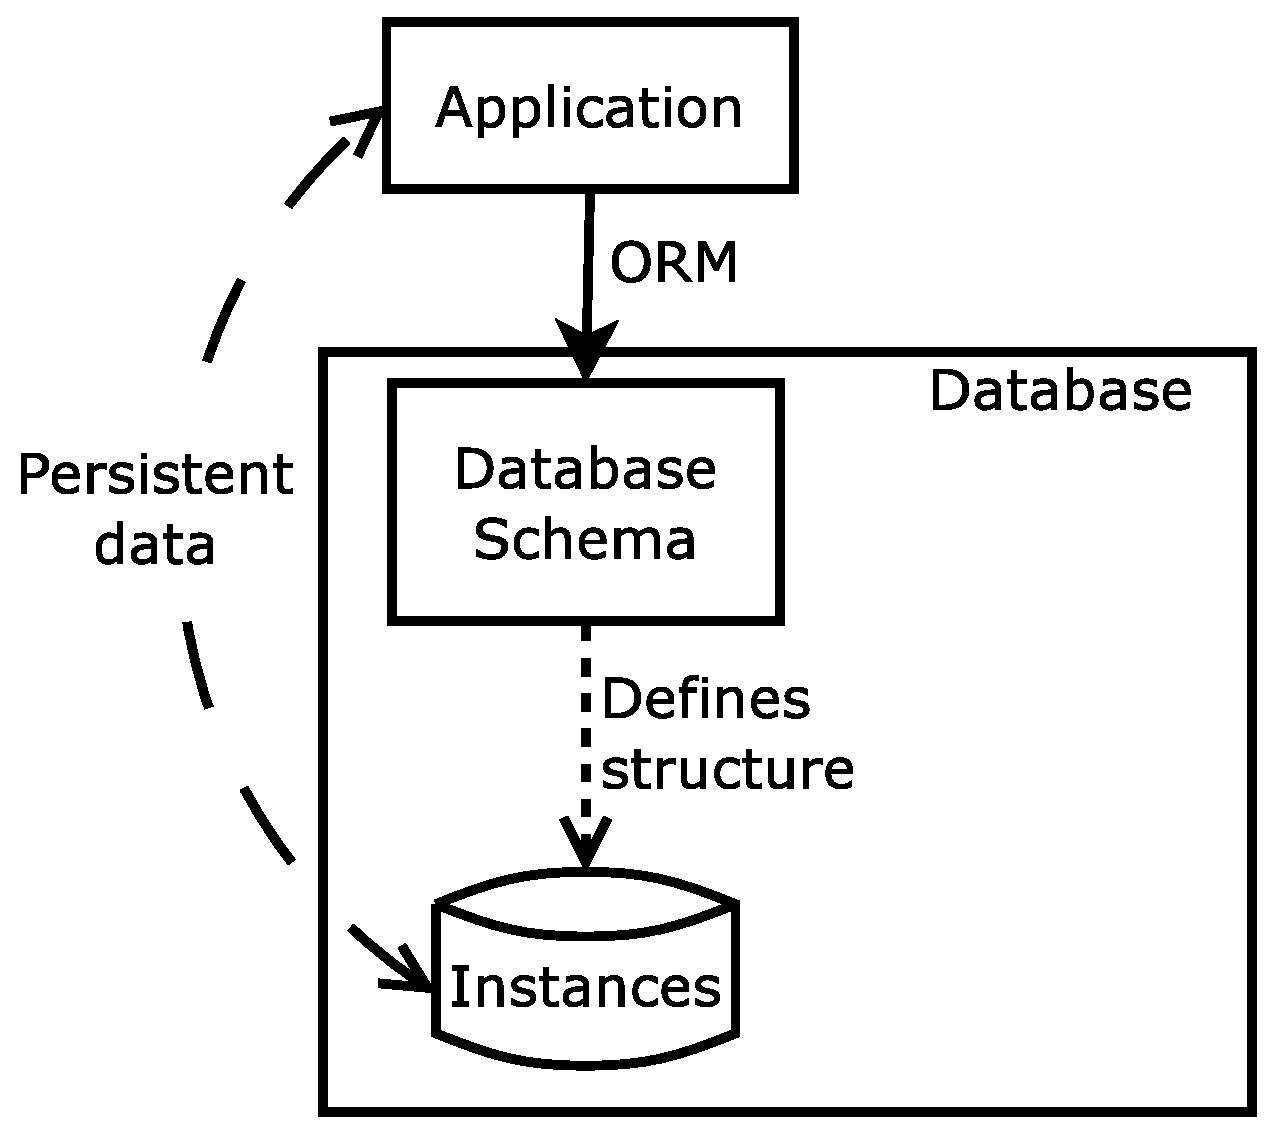
\includegraphics[scale=0.3]{./images/system}
	\caption{The model of one generation of an ORM system consists of application persistent layer and relational database for storing instances.}
\label{fig:appStructure}
\end{figure}
A software implemented in an object-oriented language, which uses relational database as a data storage is context of this paper. The situation is illustrated in the Figure \ref{fig:appStructure}. There are three important components of such a software: application (its persistent layer concretely), database (consisting of database schema and stored data) and an ORM (we will use $\rho$ as a symbol for ORM), therefore we define a software a triple:
\begin{align*}
	software = < Application, Database, \rho > \\
	sw : Applications \times Databases \times ORM \rightarrow Software \\ \\
	application : Software \rightarrow Application \\
	application(sw(a, d, \rho)) = a \\ \\
	database : Software \rightarrow Database \\
	database(sw(a, d, \rho)) = d \\
	a \in Applications, d \in Databases
\end{align*}
The software has to be in consistent state so it is beneficial for its user. The state of the software is defined to communicate the sate of the software to its user:
\begin{align*}
	state = Consistent\; s \: | \: Inconsistent \; s, \\
	s \in Softwares  \\ \\
	state : Software \rightarrow State \\
	state(s) = \begin{cases}
 		\inference{consistent(application(s)) \wedge \\ consistent(database(s)) \wedge \rho(application(s)) = database(s)}{Consistent \; s}\\ \\
 		\inference{otherwise}{Inconsistent \; s}
 	\end{cases}
\end{align*}
\subsection{Software Evolution}
\begin{figure}
\centering
	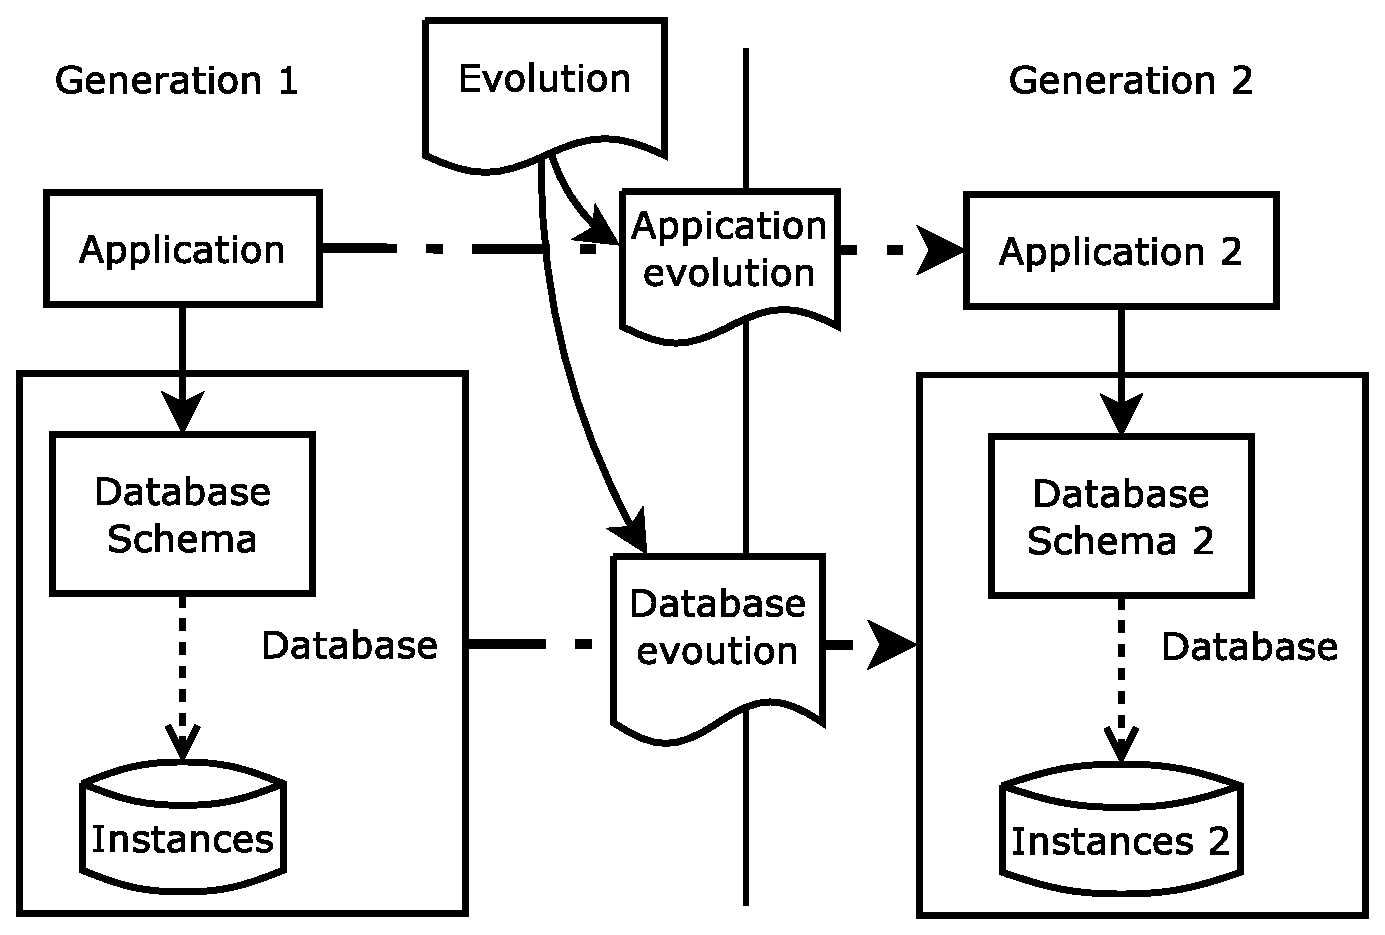
\includegraphics[scale=0.4]{./images/evolution_simple}
	\caption{The evolution of data changes the system on all levels. The figure shows all the components of the evolution process.}
	\label{fig:evolution}
\end{figure}
The evolution of a software is a transformation from one consistent state to another one. These states are called generations of the software. The evolution consists of change in application and in database as shown in the Figure \ref{fig:evolution}. We focus on situations when the evolution is initiated on the application level (as code refactoring), however the evolution has to be processed on the database level too. It means there is a set of application transformations called $AppOps$ and a set of database transformations called $DbOps$. Because there are needed different parameters for application and database evolution the set of transformation called $E$ which evolves the whole software and a mapping between $E$ and $AppOps$, respectively $DbOps$ is defined. We call this mappings $\Psi$ and $\Phi$:
\begin{align*}
\Psi : E \rightarrow AppOps \\
\Phi : E \rightarrow DbOps
\end{align*}
A subset of $E$ represents an evolution transformation of a software, which mets the first goal of our framework - a single source of data evolution for the whole software.

The application of a transformation on a software state (evolution) is marked by the $\oplus$ operator:
$$\oplus : State \times E \rightarrow State $$
and similarly the $\circ$ and the $\bullet$ operators for evolving application and database:
\begin{align*}
\circ : Application \times AppOps \rightarrow Application \\
 \bullet : Database \times DbOps \rightarrow Database
\end{align*}
The definition of the evolving operator is inspired by the monads (as used e.g. in Haskell programming language) so the state of the software can be passed from one evolution step to another, which helps us to concatenate evolution transformations.

\begin{align*}
 u \oplus t = \begin{cases}
 	\inference{u = Inconsistent \; s}{u} \\ \\
 	\inference{u = Consistent \; s}{state(sw(\Psi(u, t), \Phi(u,t))} 
\end{cases}\\ 
u \in States, t \in E, s \in Softwares
\end{align*}
\begin{align*}
 a \circ o = \begin{cases}
 	\inference{!\;consistent(a)}{a} \\ \\
 	\inference{consistent(a)}{a \circ o} 
\end{cases}\\ 
a \in Applications, o \in AppOps
\end{align*}
\begin{align*}
 d \bullet o = \begin{cases}
 	\inference{!\;consistent(d)}{d} \\ \\
 	\inference{consistent(d)}{d \circ o} 
\end{cases}\\ 
d \in Applications, o \in DbOps
\end{align*}

\section{Software Model}
The model of an ORM software consists of three parts - an application model, a database model and a ORM. The definitions of all parts assume a set $Label$ exist which contains all possible identifiers and each modeled entity is identified unambiguously identified in the model. Next there is a set $Values$ containing all possible values, which can be used in the model. 

\subsection{Application Model}
\label{sec:appModel}
The application model represents a persistent layer of an application created using object oriented language and transformations which can alter the model. 
\subsubsection{Application Structure}
Each instance is defined according to a class - the class defines the structure of its instances and relationships between them an the rest of the application. The instances are stored in the relational database in our case, therefore we define only the structure of classes in our model. Besides the structure definition, there is defined a set of functions, which allows to manipulate the application model easily. 

\begin{align*}
  \mathbf{Application} = < Class* > \\ 
  \mathbf{app} : Class* \rightarrow  Application \\ \\
  \mathbf{classes} : Application \rightarrow Class* \\
  classes(app(cs)) = cs  \\\\
  \mathbf{class} : Label \times Application \rightarrow Class   \\ 
  class(l, a) = c, c \in classes(a) \wedge name(c) = l \\ \\
  l \in Label, a = Application, cs = Class* 
\end{align*}


\paragraph{Class} represents a basic structural concept in the application model. It has a unique name, one or more properties and a class can be associated to other classes in the application. 
\begin{align*}
	\mathbf{Class} = <label, Property*, Association*> \\
	\mathbf{cl} : Label \times Property* \times Association* \rightarrow Class \\\\
% TODO association has to be only to self (all associated has to exists)
	\mathbf{name} : Class \rightarrow Label \\
	name(cl(l, props, assocs)) = l \\ \\
	\mathbf{properties} : Class \rightarrow Property* \\
	properties(cl(l, props, assocs)) = props \\ \\
	\mathbf{primitiveProperties} : Class \rightarrow Property* \\	primitiveProperties(cl(l, props, assocs)) = props', \\ props' \subset props,  \forall p \in props' : cardinality(p) \leq 1 \\ \\
	\mathbf{collectionProperties} : Class \rightarrow Property* \\	collectionProperties(cl(l, props, assocs)) = props', \\ props' \subset props, \forall p \in props' : cardinality(p) > 1 \\ \\
	\mathbf{associations} : Class \rightarrow Association* \\	associations(cl(l, props, assocs)) = assocs \\ \\
	\mathbf{associated} :  Label \times Application \rightarrow Boolean \\
  	associated(l,a) = \begin{cases}
  		\inference{\exists c \in classes(a) \wedge \exists e \in associations(c) : reference(e) = l
  	}{ true } \\
 		false
 	\end{cases} \\ \\
	l \in Label, props = Property*, assocs = Association*, a = Application
\end{align*}
	 
\paragraph{Property} represents a feature of  a class which is represented as a primitive type. The property can be mandatory, can have a default value and can represent a single value or a collection of values.
\begin{align*}
	\mathbf{Property} = <label, AppType, DefaultValue, Cardinality, Mandatory> \\ \\
	\mathbf{prop} : Label \times AppType \times String \times \mathbb{N^{*}} \times Boolean \rightarrow Property \\ \\
	\mathbf{name} : Property \rightarrow Label \\
	name(prop(l, t, val, n, m)) = l \\ \\
	\mathbf{type} : Property \times AppType \\
	type(prop(l, t, val, n, m)) = t \\ \\
	\mathbf{cardinality} : Property \rightarrow \mathbb{N^{*}} \\
	cardinality(prop(l, t, val, n, m)) = n \\ \\
	\mathbf{mandatory} : Property \rightarrow Boolean \\
	mandatory(prop(l, t, val, n, m)) = m  \\ \\
	\mathbf{owningClass} : Property \times Application \rightarrow Class  \\ 	
	owningClass(p, a) = \inference{\exists c \in classes(a) \wedge p \in properties(c)}{c}  \\ \\
	l \in Label, t \in AppType, val \in String*, n \in \mathbb{N^{*}}, m \in Boolean 
\end{align*}

\paragraph {Association} represents a connection between two classes. It has a unique name and it contains a name of the class which is referenced by the association. The class which owns the association is consider to be the starting class of an association, referenced class is consider to be the ending class of an association. The cardinalities defines the multiplicity of the association ends.
\begin{align*}
	\mathbf{Association} = <label, classRef, startCardinality, endCardinality> \\ \\
	\mathbf{assoc} : Label \times Label \times \mathbb{N} \times \mathbb{N} \rightarrow Association\\
	\mathbf{name} : Association \rightarrow Label \\
	name(assoc(l, ref, n_1, n_2)) = l\\ \\
	\mathbf{reference} : Association \rightarrow Label \\
	reference(assoc(l, ref, n_1, n_2)) = ref\\ \\
	\mathbf{startCardinality} : Association \rightarrow \mathbb{N} \\
	startCardinality(assoc(l, ref, n_1, n_2)) = n_1\\ \\
	\mathbf{endCardinality} : Association \rightarrow \mathbb{N} \\
	endCardinality(assoc(l, ref, n_1, n_2)) = n_2 \\ \\
	\mathbf{owningClass} : Association \times Application \rightarrow Class  \\
	owningClass(as, a) = \inference{\exists c \in classes(a) \wedge as \in associations(c)}{c}  \\ \\	
	l, ref \in Label,  n_1, n_2 \in \mathbb{N}, as = Association
\end{align*}


%TODO: variable types

\paragraph{AppType} represents primitive types in the application. There are usually defined types such as String, Integer, Boolean etc. in contrast there is only one type in our model, because we focus on structural and data changes and type casting operations are not important for us. The only App-Type type is called APP-STRING.
\begin{align*}
\mathbf{AppType} = APPSTRING
\end{align*}


\subsection{Database Model}
\label{sec:dbModel}
The relational database consists of database schema which defines the structure of the database and data, which in our ORM system represents instances. The database is:
\begin{align*}
	\mathbf{Database} = <table*, row*> \\ \\
	\mathbf{db} : Tables \times Rows \rightarrow Database \\ \\
	\mathbf{tables} : Database \rightarrow Tables \\
	tables(db(tabs, rs)) = tabs \\ \\
	\mathbf{rows} : Database \rightarrow Rows \\
	rows(db(tabs, rs)) = rs \\ \\
	\mathbf{table} : Label \times Database \rightarrow Table  \\
	table(l, d) = t, t \in tables(d) \wedge name(t) = l \\ \\
	tabs = Table*, rs = Row*, l \in Label, d = Database
\end{align*}


\subsubsection{Database Schema Model}
The database schema model is defined by following concepts:
\paragraph{Table} represents a basic concept of database schema. It has a unique name, one or more column and it can be related to other tables in the schema by foreign keys. Rows in the table represents stored data.
\begin{align*}
	\mathbf{Table} = <label, primaryKey, Column*, ForeignKey*>\\ \\
	\mathbf{tab} 	: Label \times PrimaryKeys \times Columns \times ForeignKeys \rightarrow Table \\ \\
	\mathbf{name} : Table \rightarrow Label  \\
	name(tab(l, pk, cols, fks)) = l \\ \\
	\mathbf{primaryKey} : Table \rightarrow PrimaryKeys  \\
	primaryKey(tab(l, pk, cols, fks)) = pk \\ \\
	\mathbf{columns} : Table \rightarrow Columns  \\
	columns(tab(l, pk, cols, fks)) = cols \\ \\
	\mathbf{foreignKeys} : Table \rightarrow ForeignKeys  \\
	foreignKeys(tab(l, pk, cols, fks)) = fks \\ \\
l \in Label, pk = PrimaryKey, cols = Column*, fks = ForeignKey*
\end{align*}

\paragraph{Column} columns define possible data values and types which can be part of a table record.
\begin{align*}
	\mathbf{Column} = <label, DbType, DefaultValue, Constraint*> \\ \\
	\mathbf{col} : Label \times DbType \times String \times Constraints \rightarrow Column \\ \\
	\mathbf{name} : Column \rightarrow Label  \\
	name(col(l, t, val, cons)) = l  \\ \\
	\mathbf{type} : Column \rightarrow DbType  \\
	type(col(l, t, val, cons)) = t  \\ \\
	\mathbf{constraints} : Column \rightarrow Constraints  \\
	constraints(col(l, t, val, cons)) = cons  \\ \\
	\mathbf{owningTable} : Column \times Database \rightarrow Table  \\
	owningTable(c, d) = \inference{\exists tab \in tables(d) \wedge c \in columns(tab)}{tab} \\ \\
l \in Label, t = DbType, val = String,\\ cons = Constraints, c = Column, d = Database
\end{align*}

\paragraph{Foreign key}
\begin{align*}
	\mathbf{ForeignKey} = <label, tableRef, Constraint*> \\ \\
	\mathbf{fk} : Label \times Label \times Constraints \rightarrow ForeignKey \\ \\
	\mathbf{name} : ForeignKey \rightarrow Label \\
	name(fk(l, tRef, cons)) = lab  \\ \\
	\mathbf{reference} : ForeignKey \rightarrow Label  \\
	reference(fk(l, tRef, cons)) = tRef  \\ \\
	\mathbf{constaints} : ForeignKey \rightarrow Constraint*  \\
	constaints(fk(l, tRef, cons)) = cons  \\ \\
	\mathbf{owningTable} : ForeignKey \times Database \rightarrow Table  \\
	owningTable(fk, d) = \inference{\exists tab \in tables(d) \wedge fk \in foreignKeys(tab)}{tab}\\\\
	l, tRef \in Label, cons = Constraint*, d = Database, fk = ForeignKey
\end{align*}


\paragraph{Primary key}
\begin{align*}
	\mathbf{PrimaryKey} =  < label > 	\\
	\mathbf{pk} : Label \rightarrow PrimaryKey
\end{align*}

\paragraph{DbType} represents primitive types in the database. There are usually defined types such as Varchar, Integer, Boolean etc. There are only two types defined in the model $DBSTRING$ as a default type of values in columns and $DBINT$ as a default type for keys.
\begin{align*}
	\mathbf{DbType} = DBSTRING \; | \; DBINT 
\end{align*}

\paragraph{Constraint} there are two types of constraints defined in the model. Both constraints are column constraints - first constraint defines unique records in a column, second constraint defines non-empty columns.
\begin{align*}
	\mathbf{Constraint} = NOTNULL \; | \; UNIQUE 
\end{align*}

%%%%%%%%%%%%%%%%%%%%%%%%%%%%%%

\subsubsection{Model of Stored Data}
A database consists not only from schema but also from data which are represented as rows in a table. A table row in our model is a tuple consisting of reference to a concrete table and a set of value pairs, which represents concrete values of concrete columns.
\begin{align*}
	\mathbf{Row} = < refTable, pair* > \\
	\mathbf{row} : Label \times Pairs \rightarrow Row \\ \\
	\mathbf{refTable} : Row \rightarrow Label \\
	refTable(row(l, ps) = l \\ \\
	\mathbf{pairs} : Row \rightarrow Pair* \\
	pairs(row(l, ps)) = ps \\ \\
	\mathbf{pairByRef} : Label \times Row \rightarrow Pair \\
	pairByRef(l,i) = \begin{cases}
		\inference{\exists p \in pairs(i) : reference(p) = l}{p} \\ \\
			\varnothing
		\end{cases}\\
	 l \in Label, ps = Pair*, i = Row
\end{align*}
The value stored in concrete column of the row is represented by pair, where the $refCol$ is a name of the column, a foreign key or its primary key and $value$ represents concrete value .
\begin{align*}
	\mathbf{Pair} = < refCol, value > \\
	[Label \times Value] \rightarrow Pair\\ \\
	\mathbf{reference} : Pair \rightarrow Label \\
	reference([l,val]) = l \\ \\
	\mathbf{value} : Pair \rightarrow Label \\ 
	value([l,val]) = val \\ \\
	l \in Label, val \in Value
\end{align*}
There functions $contains$ verify if the table contains data in context of concrete database.
\begin{align*}
	\mathbf{contains} : Table \times Database \rightarrow Boolean \\
	contains(t, d) = \begin{cases}
			\inference{\exists r \in data(d) : refTable(r) = name(t) }{true} \\ \\
		 	false
 		\end{cases} \\ \\
 l \in Label, ps = Pair*, t \in tables(d), d \in Database
\end{align*}
Each row in a database has to refer to a table in database schema and has a structure corresponding to the one defined by a table, otherwise the database is inconsistent. The consistency of database is then:
\begin{align*}
	\mathbf{consistent} : Database \rightarrow Boolean \\
	consistent(d) = \begin{cases}
 		\inference{\forall r \in data(d), \exists t \in tables(d) : reference(r) = name(t) \\ \wedge \forall p \in pairs(r) :\\ \exists u \in columns(t) \cup foreignKeys(t) : \\ reference(p) = name(u)}{true}
 	\\ \\
 	false
 \end{cases}
\end{align*}
 





\subsection{Extension of Software Definition}
The database stores instances of the application, thus the $instantiated$ function has to be defined:

$$instantiated : Class \times Software \rightarrow Boolean $$ 
\begin{equation*}
\begin{gathered}
	instantiated(c, s) = \begin{cases}
 \inference{\exists t \in tables(database(s)) : name(t) = name(c) \\ \wedge contains(t, database(s))}{true} \\ \\
  \inference{otherwise}{false} \\ \\
 \end{cases} \\ \\
 c \in classes(application(s)), s \in Software 
\end{gathered}
\end{equation*}

\subsection{Object-Relational Mapping}
\label{sec:orm}
There are defined functions for object-relational mapping used in the model in this section. The purpose of a function is indicated by its name and should be obvious from its definition. These functions do not serve for full object-relational mapping, their purpose is to help with data evolution (see Section \ref{sec:eorm}) and its propagation from application to database. However the database can be obtained from an application model by using following algorithm:

\begin{algorithmic}[1]
	\Require $a \in Application$
	\State d = Database
	\ForAll{$c \in classes(a)$} 
		\State $\rho_c(c), d$
		\ForAll{$p \in properties(c)$} 
			\State $\rho_p(p, d)$
		\EndFor
	 \EndFor
	\ForAll{$c \in classes(a)$}
		\ForAll{$as \in associations(c)$} 
			\State $\rho_{a}(as, d)$
		\EndFor
	\EndFor
\end{algorithmic}


\subsubsection{Mapping of Types}
The mapping of types assumes a bijection between application types and database types, otherwise these has to be additional information for type mapping. We focus on structural and data change therefore we simplify types and its mapping.
\begin{align*}
	\mathbf{\rho_{t}} : AppType \rightarrow DbType  \\
 	\rho_{t}(APPSTRING) = DBSTRING 
\end{align*}


\subsection{Mapping of Classes}
We assume the primary key column is created automatically by database, therefore the primary key is always created with name Id and of the $\mathbb{N^{*}}$ type and properties with cardinality 0 or 1 are mapped into columns. The associations are ignored int this mapping as it is one of the partial mapping function used in eORM.

\begin{align*}
	\mathbf{\rho_{c}} : Class*  \rightarrow Table* \\
	\rho_{c}(c) = \begin{cases}
		\inference{c = \varnothing}{\varnothing}\\\\
		\inference{|c| = 1}{table(name(c), primaryKey("Id"), \varnothing, \varnothing)}  \\ \\
		\inference{|c| > 1}{\rho_c(head(c)) \cup \rho_c(tail(c))}
 \end{cases}\\
 c = Class
\end{align*}

\subsubsection{Mapping of Properties}
There are two types of properties - the first type has cardinality 1  and it is mapped to a column. A property with cardinality greater than one has to be mapped int a table not a column, thus we have a special mapping case. When the property is mandatory the $NOTNULL$ constraint is added to the column with property value. This constraint affect already stored instances a new mandatory value has to be added to each instance.

\begin{align*}
	\mathbf{\rho_p} : Property* \rightarrow Column* \\ \\
	\rho_{sp}(p) = \begin{cases}
		\inference{p = \varnothing}{\varnothing}\\
		\inference{|p| > 1}{\rho_{sp}(head(p)) \cup \rho_{sp}(tail(p))}\\\\
 		\inference{cardinality(p) = 1 \wedge !\;mandatory(p)
 			\\ \wedge \exists t : t = table(name(owningClass(p)), d) 
		 }{\begin{gathered}
	  		column(name(p), \rho_t(type(p)), \varnothing )
		\end{gathered}} \\ \\
  		\inference{cardinality(p) = 1 \wedge mandatory(p)
			 \\ \wedge \exists t : t = table(name(owningClass(p)), d)
			\\ \wedge \not instanciated(owningClass(p))
		}{\begin{gathered}
 	 		column(name(p), \rho_t(type(p)), NOTNULL ) \\ 
		\end{gathered}}
 	\end{cases}
\end{align*}
\begin{align*}
	\mathbf{\rho_p} : Property* \rightarrow Table* \\ \\
	\rho_{cp}(p) = \begin{cases}
		\inference{p = \varnothing}{\varnothing}\\
		\inference{|p| > 1}{\rho_{cp}(head(p)) \cup \rho_{cp}(tail(p))}\\\\
     	\inference{cardinality(p) > 1 \wedge !\;mandatory(p) \\ 
     		\wedge 	\exists t : t = table(name(owningClass(p)), d)
     		}{\begin{gathered}
     			table(name(p), primaryKey("Id"), \\ column("value", 			\rho_t(type(p)), \varnothing), \\ foreignKey(name(p), 			name(owningClass(p)), NOTNULL) \\
    	\end{gathered}}\\ \\
     	\inference{ cardinality(p) > 1 \wedge mandatory(p) \\ 
     		\wedge \exists t : t = table(name(owningClass(p)), d) 
     		}{\begin{gathered}  
     			table(name(p), primaryKey("Id"), \\ 
     			column("value", \rho_t(type(p)), NOTNULL), \\ 			foreignKey(name(p), name(owningClass(p)), NOTNULL)
    	 \end{gathered}}
 	\end{cases}
\end{align*}

\subsubsection{Mapping of Associations}
A association is mapped into database as a foreign key in table representing associating class or an association can be mapped as a coupling table in case the association cardinality is M:N or 1:N.

\begin{align*}
	\mathbf{\rho_a} : Association* \rightarrow ForeignKey* \\
	\rho_a(a) = \begin{cases}
		\inference{a = \varnothing}{\varnothing}\\
		\inference{|a| > 1}{\rho_{a}(head(a)) \cup \rho_{a}(tail(a))}\\\\
		\inference{ startCardinality(a) = 0 \\ \wedge \exists t : t = table(name(owningClass(p)), d) \\ \wedge \exists u : u = table(reference(a)), d)
		}{
			foreignKey(name(a), name(t),  \varnothing) 
	 	}
  \\ \\
 	 \inference{ startCardinality(a) = 1 \\ \wedge \exists t : t = table(name(owningClass(p)), d) \\ \wedge \exists u : u = table(reference(a)), d)
 	 }{ 
		foreignKey(name(a), name(t),  NOTNULL)
	}
	 \end{cases}
\end{align*}
\begin{align*} 
	\mathbf{\rho_a} : Association* \rightarrow Table* \\
	\rho_a(a) = \begin{cases}
 		\inference{a = \varnothing}{\varnothing}\\
		\inference{|a| > 1}{\rho_{a}(head(a)) \cup \rho_{a}(tail(a))}\\\\
		\inference{  startCardinality > 1 \\ \wedge \rho(owningClass(p)) \in tables(d) \wedge \rho(reference(a)) \in tables(d)
  		}{\begin{gathered}  
		 table(name(a), pk("Id"), \varnothing, \\ foreignKey(owningClass(a),owningClass(a), NOTNULL) \\ foreignkey(reference(a), reference(a), NOTNULL)) 
  		\end{gathered}}  
 	\end{cases}
\end{align*}

\section{Model Manipulating Transformation}
\subsection{Application Transformation}
\paragraph{Add Property}Adding a property into an application structure has to verify a name collision only:
\begin{align*}
 	\mathbf{addProp} : Label \times Property \times Application \rightarrow Application \\
	addProp(l, p, a) = \inference{\exists c \in classes(a) : name(c) = l \\ \wedge \forall q \in  properties(p) : name(q) \neq name(p)}{properties(c) \cup p } \\
	l \in Label, p \in Properties, a \in Applications
\end{align*}
\paragraph{Add Association} Adding an association into an application structure has to verify if there is no name collision and if there is the associated class present in the model.
\begin{align*}
	\mathbf{addAssoc} : Label \times Association \times Application \rightarrow Application \\
	addAssoc(l, s, a) = \inference{\forall f \in associations(a) : name(f) \neq name(s) \\ \wedge \exists c \in classes(a) : name(c) = l \\ \wedge \exists k \in classes(a) : name(k) = reference(s) }{associations(c) \cup s}\\
	l \in Labels, s \in Associations, a \in Applications
\end{align*}
\paragraph{Add Class} Adding a class is limited to the case when the class has no associations, this is because it simplifies the database migration and because it is a natural way of modeling. Next the transformation $addClass$ has to verify there is no name collision
\begin{align*}
	\mathbf{addClass} : Class \times Application \rightarrow Application \\ 
	addClass(c, a) = \inference{\forall s \in classes(a) : name(s) \neq name(c) \\ \wedge associations(c) = \varnothing }{classes(a) \cup c} \\ \\
	c \in Classes, a \in Applications
\end{align*}
\paragraph{Remove Property}
\begin{align*}
 	\mathbf{remProp} : Label \times Label \times Application \rightarrow Application \\
 	remProp(l_c, l_p, a) = \inference{\exists c \in classes(a) : name(c) = l_c \\ \wedge \exists p \in properties(c) : name(p) = l_p
	}{properties(c) \setminus p }\\
	l_c, l_p \in Label, a \in Applications 
\end{align*}
\paragraph{Remove Association}
\begin{align*}
	\mathbf{remAssoc} : Label \times Label \times Application \rightarrow Application \\
	remAssoc(l_c, l_a, a) = \inference{\exists c \in classes(a) : name(c) = l_c \\ \wedge \exists f \in associations(c) : name(f) = l_a }{associations(c) \setminus f} \\
	l_c, l_a \in Labels, a \in Applications
\end{align*}
\paragraph{Remove Class} The class can be removed only in case it is not referenced by any association existing in the application.
\begin{align*}
	\mathbf{remClass} : Label \times Application \rightarrow Application \\
	remClass(l, a) = \inference{\exists c \in classes(a) : name(c) = l \\ \wedge !\: associated(c)
	} {classes(a) \setminus c }\\
	l \in Label, a = Application
\end{align*}
\paragraph{Rename Property}
\begin{align*}
	\mathbf{renProp} : Label \times Label \times Label \times Application \rightarrow Application \\
	renProp(l_c, l_o, l_n, a) = \inference{\exists c \in classes(a) : name(c) = l_c \\ \wedge \exists p \in properties(c) : name(p) = l_o \\ \wedge \forall e \in properties(c) : name(e) \neq l_n
	}{\begin{gathered}
		p.name = l_n 
	\end{gathered}}
\end{align*}
\paragraph{Rename Association}
\begin{align*}
	\mathbf{renAssoc} : Label \times Label \times Label \times Application \rightarrow Application \\
	renAssoc(l_c, l_o, l_n, a) = \inference{\exists c \in classes(a) : name(c) = l_c \\ \wedge \exists b \in associations(c) : name(b) = l_o \\ \wedge \forall e \in associations(c) : name(e) \neq l_n
	}{\begin{gathered}
		b.name = l_n 
	\end{gathered}}
\end{align*}
\paragraph{Rename Class}
\begin{align*}
	\mathbf{renClass} :  Label \times Label \times Application \rightarrow Application \\
	renClass(l_o, l_n, a) = \inference{\exists c \in classes(a) : name(c) = l_o \\ \wedge \forall e \in classes(a) : name(e) \neq l_n
	}{\begin{gathered}
		c.name = l_n \wedge \forall e \in classes(a) \\ \wedge \forall (f \in associations(e) \wedge reference(f) = l_o ) \\ : f.reference = l_n 
	\end{gathered}}
\end{align*}

\subsection{Database Transformation}
The database is composed from two separated parts - database schema and data. Several transformation are defined to make manipulating a database easily in this paper.
\paragraph{Add Column}
\begin{align*}
	\mathbf{addColumn} : Label \times Column* \times Database \rightarrow Database \\ 	
	addColum(l, c, d) = \begin{cases}
		\inference{|c| > 1}{addColumn(l, head(c), d) \bullet addColumn(l, tail(c), d)} \\ \\
		\inference{|c| = 1 \wedge \exists t \in tables(d) \wedge name(t) = l \\ \wedge \forall f \in columns(t) : name(f) \neq name(c)}{columns(t) \cup c}\\ \\
		Inconsistent \;d 
	 \end{cases}\\ 
	 l \in Label, c = Column*, d = Database
\end{align*}
\paragraph{COPY COLUMN}
\begin{align*}
	\mathbf{copyColumn} : Label \times Label \times Label \times Database \rightarrow Database \\
	copyColumn(l_s, l_t, l_c, d) = \begin{cases}
 		\inference{\exists t \in tables(d) : name(t) = l_s \\ \wedge \exists c \in columns(t) : name(c) = l_c \\ \wedge \exists e \in tables(d) : name(e) = l_t  \\ \wedge \forall q \in properties(e) : name(q) \neq l_c}{columns(e) \cup c }
	\end{cases} \\
	l_s,l_t,l_c \in Label, d = Database
\end{align*}
\paragraph{Add Table}
\begin{align*}
	\mathbf{addTable} : Table* \times Database \rightarrow Database \\ 
	addTable(t, d) = \begin{cases}
		\inference{|t| > 1}{addTable(head(t),d) \bullet addTable(tail(t), d)}
\\ \\	
		\inference{|t| = 1 \wedge \forall e \in tables(d) \wedge name(t) \neq name(e)}{tables(d) \cup c}
\\ \\
		Inconsistent \;d 
	 \end{cases}\\ 
	t = Table*,  d = Database
\end{align*}
\paragraph{Insert row}
\begin{align*}
	\mathbf{insertRow} : Row* \times Database \rightarrow Database \\
	insertRow(r, d) = \begin{cases}
			\inference{|r|>1}{insertRow(head(r), d) \bullet insertRow(tail(r), d)} \\ \\
		 	\inference{|r|=1 \wedge \exists t \in tables(d) : name(t) = reference(r) }{data(d) \cup r} \\ \\
			 Inconsistent \; d
		 \end{cases}	\\
		 r = Row*, d = Database
\end{align*}
\paragraph{Insert Values}
\begin{align*}
	\mathbf{insertValues} : Label \times Pair* \times Database \rightarrow Daatabase \\
	insertValues(l, p, d) = \begin{cases}
 		\inference{|p| > 1}{insertValues(l, head(p), d)\bullet insertValues(l, tail(p), d)}  \\ \\
 		\inference{|p| = 1 \wedge \forall e \in pairs(r_t) : reference(e) \neq reference(p) \\ \wedge \exists t \in tables(d) : name(t) = refernces(r_t), \\ \wedge \exists c \in columns(t) : reference(p) = name(c)}{pairs(r) \cup p} \\ \\
	 	 Inconsistent \; d
 		\end{cases} \\
l \in Label, p = Pair*, d = Databases
\end{align*}
\paragraph{COPY VALUES}
\begin{align*}
	\mathbf{copyValue} : Label \times Label \times Label \times (Instancece \times Instance) \times Database \times Database \\
	copyValue(l_s, l_t, l_{sc}, l_{tc} f_m, d) = \begin{cases}
 		\inference{\exists t_s \in tables(d) : name(t_s) = l_s, \\ t_t \in tables(d) : name(t_t) = l_t, \\ c \in columns(t_s) : name(c) = l_{sc}, \\ e \in columns(t_t) : name(e) = l_{tc} }{\begin{gathered}
			\forall p \in f_m(t_s, t_t)  : \\ insertValues(name(second(p)), \\ [l_{tc},value(pairByRef(l_{sc}, first(p))),d)
		\end{gathered}}
 	\end{cases}
\end{align*}



\section{Evolutionaty Transformations}
The set of all possible data evolution cases $E$ was defined in Section \ref{sec:evoIntro} together with sets $AppOps$ and $DbOps$ for evolving various layers of the software. The semantic of transformations in the set $E$ is defined by their interpretation on individual software layers. This section provides an overview of basic transformations (evolution cases) and theirs interpretation on the application and the database. The section starts with simple transformations as the complex one can be often implemented as theirs concatenation. The transformations are divided into three groups - first group creates the structure of a software, second group removes parts of a software structure and third group is able to alter the structure.

The definition of a transformation consists of two parts - a conditions of transformation feasibility and its impact on the context (application or database). If the conditions of feasibility are not met, the transformation cannot change the context - the software cannot evolve.  We decide to use following transcription to cover all aspects of transformation definition:
\begin{align*}
operation(parameters, context) = \begin{cases}
  \inference{conditions \; of \; feasibility}{impact \; on \; context}\\ \\
  \inference{otherwise}{context}
 \end{cases}
\end{align*}
The second branch of the operation definition is an implicit assumption - if an operation is not feasible in a software, its state become inconsistent. We will not state this implicit assumption in the operations definitions to increase theirs readability.


\subsection{Software Creation}
There are defined three transformations which are able to create a software: $newClass$, $addProperty$, $addAssociation$. These three transformations can be used to create a software from a scratch. The first of them has no impact on stored data, whereas the rest of them can in some cases.
\begin{align*}
\mathbf{addProperty} : Label \times Property \times State \rightarrow State \\
\Psi(s, addProperty(l, p)) = application(s) \circ addProp(l,p) \\
\Phi(s, addProperty(l, p)) = database(s) \bullet insertProp(l, p) \\
s \in Softwares, l \in Label, p \in Properties
\end{align*}

Whereas the $insertProp$ on database level can change stored data too, because a mandatory property can be added into a class with already existing instances, then a default value has to be added to all existing instances.
\begin{align*}
insertProp(p, d) = \begin{cases}
\inference{!\:mandatory(p) \vee !\:instantiated(owningClass(p))}{addColumn(l, \rho(p,d), d)} 
\\ \\ 
\inference{ \wedge mandatory(p) \vee instantiated(owningClass(p)) \\ \wedge cardinality(p) \leq 1}{\begin{gathered} addColumn(l, \rho(p,d), d) \\ \bullet \forall r \in data(d), reference(r) = name(t) : \\ appendValue(name(t), [name(p), defaultValue(p)], d)
\end{gathered}
} 
\\ \\
\inference{ \exists t \in tables(d) : name(t) = name(owningClass(p)) \\ \wedge mandatory(p) \wedge instantiated(owningClass(p)) \\ \wedge cardinality(p) \leq 1}{\begin{gathered}
addTable(\rho(p,d), d) \bullet \forall r \in row(owningClass(p)) :\\ insertRow(row(name(p), ["value", defaultValue(p)], \\ [name(p), value(primaryKey(r))]),d) 
\end{gathered}
} 
\end{cases}\\
p \in Properties, d \in Dataabses
\end{align*}

\begin{align*}
\mathbf{addAsociation} : Label \times Association \times (Row \times Row) \times State \rightarrow State \\
\Psi(s, addAsociation(l, a, f_m)) = application(s) \circ addAssoc(l, a) \\
\Phi(s, addAsociation(l, a, f_m)) = database(s) \bullet insertAssoc(l, a, f_m)
\end{align*}

Adding an association into a database is complicated because of already existing instances. When an association between classes is added the instances of both classes has to be paired. This pairing is provided by the function $f_m$:
$$f_m : \rightarrow Instance \times Instance $$

\textbf{TODO: define the features of the $f_m$ function}

The $insertAssoc$ function is defined as:
\begin{align*}
insertAssoc : Association \times Database \times (Row \times Row) \\
insertAssoc(a, d, f_m) = \begin{cases}
\inference{ \exists t_s, t_t \in tables(d) : name(t_s) = name(owningClass(a)) \\ \wedge name(t_t) = reference(a) \\ \wedge \not \exists f \in foreignKeys(t_t) : name(f) = name(a) \\ startCardinality(a) \leq 1}{\begin{gathered}
addForeignKey(name(t_s), \rho(a,d), d) \\ \bullet \forall r \in f_m(owningClass(a), reference(a)) : \\ insertRow(row(name(t_s), [name(a), \\ value(primaryKey(first(r)))]), d)
\end{gathered}
 }
 \\ \\
\inference{ \exists t_s, t_t \in tables(d) : name(t_s) = name(owningClass(a)) \\ \wedge name(t_t) = reference(a) \\ \wedge \not \exists f \in foreignKeys(t_t) : name(f) = name(a) \\ startCardinality(a) > 1}{\begin{gathered} addTable(\rho(a,d),d) \\ \bullet \forall r \in f_m(owningClass(a), reference(a)),\\ t \in tables(d) : name(t) = name(a) : \\ insertRow(row(name(a), [name(t_s), \\ value(primaryKey(first(r)))] [name(t_t), \\ value(primaryKey(second(r)))]), d)
\end{gathered}
 } 
 \end{cases}\\
 a \in Associations, d \in Databases
\end{align*}

\begin{align*}
\mathbf{newClass} : Class \times State \rightarrow State \\
\Psi(s, newClass(c)) = application(s) \circ addClass(c) \\
\Phi(s, newClass(c)) = database(s)  \bullet addTable(\rho(c,d), d) \\ \bullet addColumn(name(c), \{\forall r \in singleProperties(c) | \rho(r,d)\}, d) \\ \bullet addTable(name(c), \{\forall r \in collectionProperties(c) | \rho(r,d)\}, d)  
\end{align*}

\paragraph{Add Class} The $insertClass$ operation changes the structure of the database schema only, because the $insertAssoc$ transformation needs a mapping function to work properly, which is not part of the $newClass$ definition. The situation reflect the modeling praxis when the structure of a class is defined and then it is associations are created.
%\begin{align*}
%insertClass : Class \times Database \rightarrow Database \\
%insertClass(c, d) = \inference{ \forall t \in tables(d) : name(t) \neq name(\rho(c)) \\
%	%\forall a \in associations(c), \exists u \in  tables(d) : reference(a) = name(u) \\ 
%	assocaiations(c) = \varnothing
%}{
%\begin{gathered}
% addTable(\rho(c, d),d) \\ \wedge t \rho(singleProperties(c)) \wedge \rho(collectionProperties(c)) \\ 
%\end{gathered}
%}
%\end{align*}



\subsection{Software Decomposition}
\begin{align*}
RemoveClass: Label \times Software \rightarrow State  \\
\Psi RemoveClass(l, s) = applications(s) \circ remClass(l) \\
\Phi RemoveClass(l, s) = database(s) \bullet dropClass(l) \\
\\ l \in Label, s \in Software 
\end{align*}
\begin{align*}
dropClass(l,d) = \inference{ \exists t \in tables(d) : name(t) = l  \\ \wedge \not \exists r \in data(d) : owningTable(r) = l \\  \not \exists j \in tables(d) \wedge f \in foreignKeys(j) : reference(f) = l }{ tables(d) \setminus \rho(c)}
\end{align*}

\begin{align*}
RemoveProperty: Label \times Label \times State \rightarrow State \\
\Psi RemoveProperty(l, l_p, s) =  applications(s) \circ  remProp(l, l_p) \\
\Phi RemoveProperty(l, l_p, s) =  database(s) \bullet dropProp(l, l_p) \end{align*}
\begin{align*}
dropProp(p, d) = \begin{cases}
 \inference{ \exists t \in tables(d) : name(t) = name(owningClass(p)) \\ \wedge \exists c \in columns(t) : name(c) = name(p) \\ \wedge \not \exists r \in data(d) : owningTable(r) = name(owningClass(p)) }{columns(t) \setminus c
} \\ \\
  \inference{ \exists t \in tables(d) : name(t) = name(owningClass(p)) \\ \wedge \not \exists c \in columns(t) : name(c) = name(p) \\ \wedge \exists u \in tables(d) : name(u) = name(p) \\ \wedge \not \exists r \in data(d) : owningTable(r) = name(owningClass(p))}{ tables(d) \setminus u }
 \end{cases}
\end{align*}

\begin{align*}
RemoveAssociation : Label \times Labels \times State \rightarrow State \\ 
\Psi RemoveAssociation(l, l_a, s) = application(s) \circ remAss(l, l_a) \\
\Phi RemoveAssociation(l, l_a, s) = database(s) \bullet dropAssoc(l, l_a) \\
l_c, l_a \in Labels, a \in Applications
\end{align*}
\begin{align*}
dropAssoc(l, l_a, d) =  \begin{cases}
 \inference{\exists t \in tables(d) : name(t) = l
 \\ \wedge \exists f \in foreignKeys(t) : name(f) = l_a
 \\ \wedge \forall r \in data(d) : owningTable(r) \neq t}{ foreignKeys(t) \setminus f }
 \\ \\
 \inference{\exists t \in tables(d) : name(t) = l_a
 \\ \wedge \exists f \in foreignKeys(t) : name(f) = l
 \\ \wedge \forall r \in data(d) : reference(r) \neq t}{ tables(d) \setminus t}
 \end{cases}
\end{align*}



\subsection{Software Alternation}
\paragraph{Rename Class}
\begin{align*}
RenameClass : Label \times Label \times State \rightarrow State \\ 
\Psi(RenameClass(l_o, l_n), s) = application(s) \circ renClass(l_o, l_n) \\
\Phi(RenameClass(l_o, l_n), s) = database(s) \bullet alterClass(l_o, l_n) \\ \\
\end{align*}

\begin{align*}
alterTable:  Label \times Label \times Database \rightarrow Database \\
alterTable(l_o, l_n, d) = \inference{\exists t \in tables(d) : name(d) = l_o \\ \wedge \forall e \in tables(d) : name(e) \neq l_n}{\begin{gathered}
t.name = l_n \\ \wedge \forall e \in tables(a) \wedge \forall (f \in fks(e) \wedge reference(f) = l_o ) \\ : f.reference = l_n 
\end{gathered}}\\
l_o, l_n \in Label, s \in States, a \in Applications, d \in Databases
\end{align*}

\paragraph{Rename Property}
\begin{align*}
	RenameProperty : Label \times Label \times Label \times State \rightarrow State \\ \\
\Psi(RenameProperty(l_c, l_o, l_n, s)) = application(s) \circ renProp(l_c, l_o, l_n) \\
\Phi(RenameProperty(l_c, l_o, l_n, s)) = database(s) \bullet alterColumn(l_c, l_o, l_n) \\\\
\end{align*}

\begin{align*}
alterColumn : Label \times Label \times Label \times Database \rightarrow Database \\
	alterColumn(l_c, l_o, l_n, d) = \begin{cases}
 \inference{\exists t \in tables(a) : name(t) = l_c \\ \wedge \exists c \in columns(t) : name(c) = l_o \\ \wedge \forall e \in columns(t) : name(e) \neq l_n}{\begin{gathered}
c.name = l_n 
\end{gathered}}
\\ \\
\inference{\exists t \in tables(a) : name(t) = l_o \\ \wedge \forall e \in tables(t) : name(e) \neq l_n}{\begin{gathered}
t.name = l_n 
\end{gathered}}
 \end{cases}
 \\
l_c, l_o, l_n \in Label, a \in Applications, s \in States, d \in Databases
\end{align*}

\paragraph{Rename Association}
\begin{align*}
RenameAssociation : Label \times Label \times Label \times State \rightarrow State \\
\Psi(RenameAssocaiation(l_c, l_o, l_n), s) = application(s) \circ renAssoc(l_c, l_o, l_n)\\
\Phi(RenameAssocaiation(l_c, l_o, l_n), s) = \begin{cases}
	\inference{\mathbf{TODO}}{database(s) \bullet alterTable(l_c, l_o, l_n)}
 \\
  \inference{\mathbf{TODO}}{database(s) \bullet alterColumn(l_c, l_o, l_n)}
 \end{cases}
\\\\
alterColumn : Label \times Label \times Label \times Database \rightarrow Database \\
%	alterAssoc(l_c, l_o, l_n, d) = \begin{cases}
%?? \inference{\exists t \in tables(a) : name(t) = l_c \\ \wedge \exists f \in fks(t) : name(c) = l_o \\ \wedge \forall e \in fks(t) : name(e) \neq l_n}{\begin{gathered}
%f.name = l_n 
%\end{gathered}}
%\\ \\
%\inference{\exists t \in tables(a) : name(t) = l_o \\ \wedge \forall e \in tables(t) : name(e) \neq l_n}{\begin{gathered}
%t.name = l_n 
%\end{gathered}}
% \end{cases}
% \\
l_c, l_o, l_n \in Label, a \in Applications, s \in Sates, d \in Databases
\end{align*}


\paragraph{Copy Property}
All transformations described earlier does change mostly the structure of a application only. Therefore we define  the transformation for copying a property from one class to another. To copy property is the basic way to move data from instances of a class to instance of another class. Note the transformation does not move a single value, but it move the values for all instances in the software.

The copy property can be implemented as a transformation composed by operations for adding and removing property, nevertheless this composition would not work with instances, where the $copyData$ transformation is used.
\begin{align*}
	\mathbf{CopyProperty} : Label \times Label \times Label \times (Instance \times Instance) \times State \rightarrow State \\
	\Psi(CopyProperty(l_s, l_t, l_p, f_m), s) = \inference{\exists c \in classes(a) : name(c) = l_s \\ \wedge \exists p \in properties(c) : name(p) = l_p }{application(s) \circ addProp(l_t, p)} \\
	\Phi(CopyProperty(l_s, l_t, l_p, f_m), s) = \begin{cases}
		\inference{\mathbf{TODO}}{\begin{gathered}
			database(s) \bullet copyColumn(l_s, l_t, l_p) \\ \bullet copyValues(l_s, l_t, l_p, f_m) 
			\end{gathered}} \\ \\
		\inference{\mathbf{TODO}}{\begin{gathered}
			database(s) \bullet copyTable(l_s, l_t, l_p) \\ \bullet copyRows(l_s, l_t, l_p, f_m) 
			\end{gathered}}
 \end{cases}
\end{align*}

With a copy property transformation defined we are able to define advanced evolution scenarios.

\paragraph{Change Cardinality}
$$\rho_{CcP} : Property \times \mathbb{N^{*}} \times Application \rightarrow Property $$
$$\rho_{cardA} : Association \times \mathbb{N^{*}} \times Application \rightarrow Association $$

\section{Conclusion}



\end{document}


%	CopyProperty(l_s, l_t, l_p, a) = \inference{\exists c \in classes(a) : name(c) = l_s \\ \wedge \exists p \in properties(c) : name(p) = l_p \\ \wedge \exists e \in classes(a) : name(e) = l_t  \\ \wedge \forall q \in properties(c) : name(q) \neq l_p}{\begin{gathered}
%properites(e) \cup p 
%\end{gathered}}


% This is important in case we have an evolution consisting of several evolution operations. These operations has to be proceed in concrete order and all of them has to change the software otherwise the software can become inconsistent from user point of view (the structure or stored data will not correspond with the users' reality). To assure the right behavior of evolution operations and to propagate operations fail to the user we extend the definition of a software to make it a monad. The extension consists in defining a software state and operations $ret$ and $\oplus$ (called evolve), which is used as a concatenation of operations as well.
%
%Each evolution transformation has a definition: $Software \rightarrow State$ and all evolution transformations creates a set called $Transformations$, then a concatenation of evolution transformation is defined as:
%\begin{equation*}
%\begin{gathered}
% \oplus : State \times Transformations \rightarrow State  \\ \\
% u \oplus t = \begin{cases}
% u, \; u = Inconsistent \; s \\
% t(u), \; u = Consistent \; s 
%\end{cases}\\ 
%u \in States, t \in Transformations, s \in Softwares
%\end{gathered}
%\end{equation*}
%
% To describe these two aspects od software evolution we decide to define transformations for each layer separately. The separation of transformation contexts help us to define transformation specific for application or database evolution, which can ease both - understanding and defining the transformation. The transformations specific for a context are called operations and they creates two sets- first one for application evolution: $AppOps$  and second one for database evolution $DbOps$. Applying of a transformation is defined:
%\begin{align*}
%u \oplus t = ret(<application(u) \oplus o_{app}, database(u) \oplus o_{db}>) \\
%u \in Softwares, t \in Transformations, o_{app} \in AppOps, o_{db} \in DbOps
%\end{align*}